\section{Background} \label{background}

A literature study has been conducted to situate the thesis topic. Multiple subjects lay at the base of the design described in section \ref{design}. First, the switch to, the components, and types of electronic health record systems are described. Next three key subjects are explained in the following order: chronic diseases, telemonitoring, and dashboard design. The last section mentions the issues surrounding medical data privacy and standards. 

    % waarom belangrijk om te beschrijven
    \subsection{Electronic health record systems}

    Health information systems are becoming an important part of health care. They support patient care as well as administrative and financial tools. At the heart of these systems lies the electronic health record. An electronic health record (EHR) is a repository of electronically maintained information about an individual's health status and health care, stored such that it can serve multiple legitimate uses and users of the record \cite{biomedical_informatics}. An electronic health record system (EHRS) provides tools to manage and interact with these records. These tools include reminder generation, data analysis, and decision support. It helps the clinician to organize, interpret and react to medical data.

    The first section describes the transition from paper-based records to digital and its implications for the medical world. A summary of the main components present in an EHRS is described in the next section. The functionality of an EHRS can be categorized into two types: a monolithic system tries to provide more general care, while smaller and more specialized systems cater to more specific types of care. The last section compares the two types and highlights the benefits and drawbacks of both.

    No existing EHRS were reviewed. Access to these systems is limited to open-source solutions as most are purchased under a license. Consequently, reviews of these systems are difficult to find as institutions only purchase software after thorough review of its features. Only one article was found which compared three open-source health systems \cite{de2012overview}. However, no literature was found for proprietary systems.

        % signify importance
        \subsubsection{Moving away from paper} \label{2_ehrs_paper}

        For modern medicine, the traditional paper-based medical records are not suited in today's world filled with technology. The drawbacks of information on paper are obvious when compared to digitally stored information.

        \paragraph{Functionality} Digital records allow systems to aggregate, process and create statistics of the data it contains. For example, a system can generate heart rate graphs with statistics, summarizing many values. If the user hovers over a data point in the graph, the exact value is shown. Printed tables and graphs showing the same data lack this interaction. Also, more effort is required from the clinicians, as data is scattered across multiple paper-records.

        A paper-based medical dossier can store for example medical images, such as x-rays. Compared to a digital image, paper loses a lot of detail. As such, other multimedia types cannot be stored on paper, while a digital record can. An EHRS can provide tools to interact with all these types of file formats.

        In terms of data input, an EHRS can detect and prevent false data input. The system can make sure all necessary data fields filled in and in the correct format. This results in more complete and accurate data gathering with fewer errors.

        \paragraph{Information quality} A summarizing paper noted that the use of EHRS leads to more complete, accurate, comprehensive, and reliable data compared to paper-based records \cite{ehrs_summary}. As mentioned in the previous paragraph, a digital system can impose rules on data fields to avoid missing or entering the wrong data. In terms of comprehensibility, poor handwriting leads to wrong or loss of information, which digital systems avoid.

        \paragraph{Accessibility} Paper records are difficult to access because most of the time only one copy exists. Therefore, transferring these records to other branches or institutions is difficult: the record has to be found in the often large medical dossier, has to be copied and then manually sent. Also, misfiling, flooding or fires lead to irrecoverable loss of the data. Creating backups of the digital records avoids the last issue, but difficulties surrounding data transfer are still present. Most institutions have their own database structures which hinders the transfer of raw data. To remedy this, IT staff has to create an interface to read the data. Sending for example PDF-reports via email is a convenient alternative, although limited in functionality compared to paper records.

        Moving data from paper to a digital format requires a lot of manual work. While automation is possible, such as scanning and processing the paper forms with software, verification is still necessary. All the data fields from the documents need to find a place in the EHR, which frequently is not possible. Extra diagnostic information scribbled all over the the document, will be lost for example. Also, what do we do with unreadable data due to poor handwriting? What happens with two forms which contain partly the same information? Do we save the information twice or do we add extra checks? Because of these reasons, adopting an EHRS is a significant undertaking for an institution. As such, the benefits are not immediately apparent.

        Because digital storage increases accessibility significantly, security measurements have to be taken. If not, data can be stolen, deleted or even altered, which means a breach of privacy (see section \ref{2_privacy}. This also adds to the complexity of developing EHRS. 

        \paragraph{Efficiency} An important task of an EHRS is to facilitate effective care. An early study saw a 6\% increase in productivity when EHRS were deployed in health care institutions \cite{ehrs_efficiency}. However, other factors are at play, such as the adoption rate. The transition from paper-based documenting to digital is accompanied by a learning curve, which can be steep. After the switch, the productivity will most likely be lower at the start. As the users become more experienced with the software, it will increase. Today most institutions have already made the transition to an EHRS, so this has become less of an issue.

        \subsubsection{Components of an EHRS} \label{ehrs_components}

        As mentioned before, EHRS do not simply store patient records. They consist of many components which ultimately defines how well they perform in health care. Literature defines many lists of components which should be essential. However, we list the following five components as key \cite{biomedical_informatics}:

        \paragraph{Integrated view of patient data} An EHR must allow storage of a wide range of data types. This can be text, numbers, images, video, and others. Some data can still be on paper due to lacking support of the EHRS, as mentioned in section \ref{2_ehrs_paper}. To display more complex data types, such as x-ray images, standards are used. A brief overview of medical standards is described in section \ref{2_standards}.

        \paragraph{Clinician order entry} The point at which the clinician enters treatment instructions is called order entry. An order entry system assists the clinician during the decision-making process to ensure the instructions are correct. It also reduces errors and costs compared to paper order entry for the same reasons already mentioned in section \ref{2_ehrs_paper}.

        \paragraph{Clinical decision support} A decision support system embed into an EHRS aids the clinician by suggesting certain actions when certain situations occur. If for example, a patient is due for vaccination, the system notifies the clinician by presenting a constructed order which needs to be confirmed or denied. The system can do this for a bulk of patients, so manual checkups are not required, thus saving time.

        \paragraph{Access to knowledge resources} During the writing of notes or orders for a patient, clinical questions often arise. Instead of asking colleagues or searching through multiple manuals, the EHRS can search for relevant literature to address the question. Due to the internet, a very large source of information is readily available.

        \paragraph{Integrated communication and reporting support} Communication is an important part of health care. Often clinicians spread across multiple institutions provide care for the same patient. Communication, therefore, directly affects the effectiveness of patient care. Tools that easen and simplify this process are essential for a health system. 

        Most institutions are bound by their own EHRS. If data resides in another institution's health system, then access has to be requested. Health Information Exchange removes the need to manually ask for data access as institutions are able to reach beyond their own system. This, however, needs to be supported by the institution.\\
        
        \noindent Throughout the years, many EHRS have been developed which may or may not integrate all of the above components. Should an essential component be missing, an institution may add another software system. This has its own benefits and drawbacks.

        \subsubsection{Monolithic vs. multiple EHRS} \label{ehrs_comparison}

        Health care institutions can opt for a monolithic EHRS or combine multiple EHRS to achieve all required functionality. There advantages and drawbacks to both \cite{multiple_ehrs}. Elements that influence this choice include IT infrastructure, safety risks, the volume of care and frequency with which patients move facilities. It is possible that a single EHRS does not satisfy the requirements of an institution. A reason for this is that certain branches require specially tailored software for their clinical practice, which the current EHRS in use lacks.

        Functionality wise, a monolithic EHRS tends to appeal to more general types of care, whereas it lacks in very specific ones. Also, vendors that offer these all-in-one solutions have less experience with these special types of care which reduces the chance it will be added to the system. Vendors of specific EHRS do have this expertise and can tailor the system to the needs of the customer. In this case, combining a system that supports general care with special care systems seems like the best choice. However, other factors have to be considered.

        The advantage of a monolithic system is that the data it uses is centralized. This ensures that all data is accessible anywhere throughout the system and is easier to maintain. When multiple systems are in place, data has to be exchanged between them. As a result, searching for data is more difficult. As mentioned in section \ref{2_ehrs_paper}, due to different data structures, data exchange is difficult. To solve this issue, an intermediate EHRS can be developed. This system serves solely for the purpose of data collection and transformation. All other systems search for data in this intermediate system. However, this leads to another system, requiring additional costs, development effort, and maintenance.
    
    % algemene beschrijving
    % welke 4 + varianten
    % beschrijving met behandeling en problemen, oorzaken, cijfers, kosten...
    \subsection{Chronic diseases} \label{chronic_diseases}
    A chronic disease can be defined as a long-lasting human health condition. If the length of the condition is at least three months, the term chronic is used. The World Health Organization defines four major categories of chronic diseases: cardiovascular diseases, cancer, diabetes and chronic obstructive pulmonary disease \cite{world2017noncommunicable}. Cardiovascular disease is the leading cause of death worldwide \cite{mendis2011global}. Combined with cancer, they accounted for 46\% of all deaths in the United States in 2015 \cite{national2016health}. Also, 86\% of all health care spending of 2014 was for patients with one or more chronic conditions \cite{gerteis2014multiple}.

    We now briefly define each disease category. All diseases that involve the heart or blood vessels belong to the cardiovascular disease group. Typical examples of such diseases are stroke and coronary artery disease. Cancer has many different variants, but all of them share the same behavior. This is when some cells of the human body start to divide without stopping and that it spreads to surrounding tissues \cite{cancer_def}. Diabetes is a disease group in which there are high blood sugar levels present for a prolonged period of time. There are three types of diabetes: type 1, type 2, and gestational diabetes. Lastly, chronic obstructive pulmonary disease (COPD) is a chronic lung disease that is characterized by persistent respiratory symptoms and airflow problems \cite{vogelmeier2017global}. Examples of these symptoms are shortness of breath and coughing. The worsening of these symptoms for a period of time is called an acute exacerbation.
    
    The following sections give more information on the prevention and management of these diseases.

        \subsubsection{Prevention}

        The factors to lower the incidence of chronic diseases mainly involve lifestyle and diet changes \cite{willett2006prevention}. We summarize the recommended changes as follows:
            \begin{itemize}
                \item Avoid smoking: prevent cardiovascular disease, diabetes type 2, cancer, and COPD. Secondhand smoking also contributes significantly to the risk of chronic diseases \cite{us2006health}.
                \item Maintain a healthy weight: prevent cardiovascular disease, diabetes type 2, and cancer. One should aim for a BMI between 18.5 to 25, ideally less than 23. The next two items help achieving this.
                \item Maintain daily physical activity and limit time spent sedentary: prevent cardiovascular disease, diabetes type 2, and colon and breast cancer. A healthy goal is to perform physical activity for at least half an hour a day. Sedentary activities such as watching television should be limited to maximum two hours a day.
                \item Eat a healthy diet: prevent cardiovascular disease, diabetes type 2, and some types of cancer. Some factors that attribute to a healthy diet are as follows: consume healthy fats, eat plenty of fruit and vegetables, replace refined grains with whole grains, limit sugar intake, limit excessive calories, and limit sodium intake.
            \end{itemize}

        \noindent The aforementioned lifestyle and dietary changes are closely coupled as they affect one another. Eating healthy is an important step of losing weight. However, solely changing diet without exercising can limit progress. 

        Although one can argue that the incidence of chronic diseases is largely dependent on genetics, it was estimated that 90\% of cardiovascular disease can be prevented \cite{mcgill2008preventing}. This calls for the need to make the general public aware of implementing these lifestyle changes. Programs that promote cycling or walking to school or the workplace are, for example, a manner to engage in physical activity.

        % patient education
        \subsubsection{Management}

        \begin{figure}[!t]
            \centering
            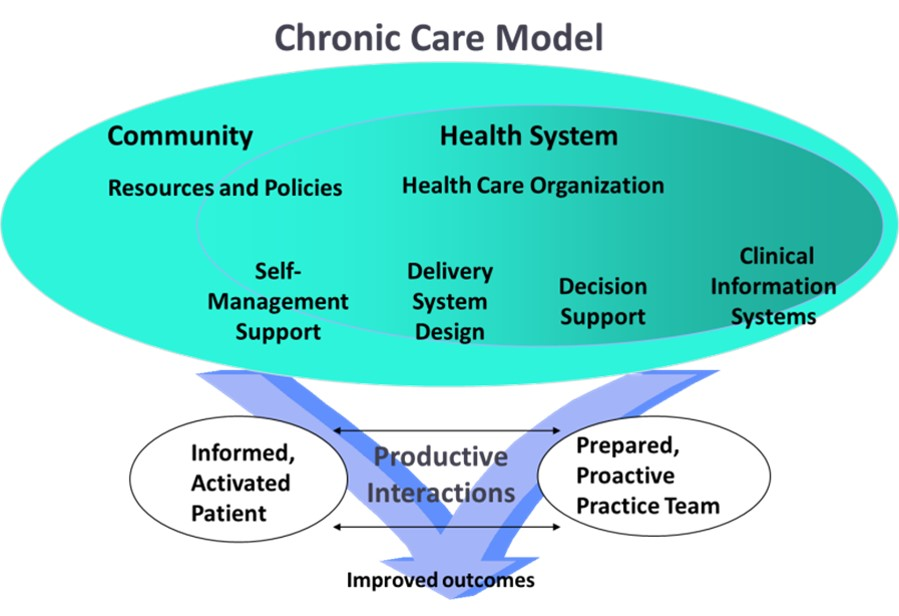
\includegraphics[width=0.8\textwidth]{chapters/2_background/chronic_model}
            \caption{Chronic Care Model}\label{fig:chronic_care}
        \end{figure}

        The Chronic Care Model was designed to improve the quality of chronic disease management for primary care \cite{bodenheimer2002improving}. The model recognizes six essential elements in chronic care, which figure  summarizes:
        \begin{itemize}
            \item Community resources and policies: mobilize community resources to meet the needs of patients. Education classes, self-help groups, and exercise programs are examples of such resources.
            \item Health care organization: create an organization that provides safe and high quality care. 
            \item Self-management support: patients need to be trained and given the necessary tools to effectively self-manage their chronic disease.
            \item Delivery system design: alter the structure of the medical practice to assure effective care and self-management support.
            \item Decision support: promote care consistent with scientific data and patient preferences.
            \item Clinical information system: organize data to facilitate effective care.
        \end{itemize}

        \noindent Improvements in chronic disease management and reduced health care costs have been observed after implementing this model. \cite{bodenheimer2002improving_2}. Of these elements, most studies focus on self-management support interventions \cite{reynolds2018systematic}. The same lifestyle and dietary changes mentioned in the previous section are applied by the patients, paired with following a medication plan. However, one key aspect of self-management is patient education as it affects the patients perception of effectiveness of the intervention \cite{wallace2010influence}. Self-management is heavily facilitated through telemonitoring, which the next section covers.

    \subsection{Telemonitoring} \label{2_telemonitoring}
    % between consultations
    % in relation to EHRS
    % transfers burden partly to patient
    Monitoring patients at a distance through the use of information technology is called telemonitoring \cite{systematic_review}. Here, the patient uses special monitoring devices to gather data which in turn is sent to the health care provider. While many health conditions can be monitored, telemonitoring is most prevalent in chronic disease management discussed in the previous section. A study showed that the complications of chronic diseases and costs can be reduced by the use of telemonitoring. Also, care can be provided without the use of hospital beds and the time spent managing the disease is lower \cite{telemonitoring_current_state}.

    To get a better understanding of telemonitoring, an overview of the its application to chronic disease management is given. Second, the difficulties surrounding telemonitoring are mentioned.

        \subsubsection{Chronic disease management}
        A lot of studies have been conducted to test the effect of telemonitoring on chronic disease management. For all but one of the four disease categories mentioned in section \ref{chronic_diseases}, general literature was found: the literature found on cancer focussed on very specific types of the disease and not in the general sense. Consequently, only the application of telemonitoring on the other categories is discussed.

        \paragraph{Cardiovascular diseases} One study recruited 390 patients to test the effect of telemonitoring to reduce hospital days and total costs \cite{tompkins2010randomized}. 193 individuals in the intervention group were to take daily measurements using special hardware. The hardware recorded the weight, blood pressure, heart rate and blood oxygen levels. Diabetes patients received an additional blood glucose meter. Patients were also required to fill in a predetermined set of questions every week. On the clinician's end, nurses were shown a summarizing table indicating if the sent results were good, bad or missing. Based on these results, the nurses decided to contact the patient if extra care was required.

        The study concluded that telemonitoring appears to facilitate more efficient outpatient care and potentially reduce costs. The total numbers of hospital days for the patients in the intervention group showed a tendency to be lower and fewer emergency department visits. However, there were more urgent care and primary care visits.

        Another research paper reviewed 30 studies and noted that most patients had a positive experience and little difficulty with telemonitoring technology \cite{inglis2010structured}. In total there were more than 9500 patients in the studies. The summary concluded that there were fewer deaths, fewer hospital admissions and improved quality of life. There were also hints of reduced cost, but some studies did not report on this topic. None of the studies reported on the optimal duration of for telemonitoring.
        
        The effect of telemonitoring treatment on cardiovascular patients is still unclear. A paper criticized the aforementioned one, stating that the conclusions made were only valid for small studies. For large trail studies, there was no significant effect \cite{chaudhry2010telemonitoring}.

        \paragraph{Diabetes} Due to the majority of research reporting on telemonitoring for diabetes type 2, type 1 will not be considered in the scope of this thesis. Due to it being a long-term disorder, combining the management of diabetes with telemonitoring is well documented in literature.

        One study required 32 patients to take blood glucose measurements for nine months using a Bluetooth capable glucose meter. The meter sent the measurements to a mobile phone which in turn forwarded them to a hospital server. Based on the measurements clinicians would review them and send recommendations to the patient and their general practitioner. The results showed a decrease in HbA\textsubscript{1C} from 8.40\% to 7.76\%. Due to the low amount of patients, the final conclusion said that the benefit of telemonitoring would likely be small \cite{istepanian2009evaluation}.

        Diabetes also has an effect on blood pressure, as approximately 50 to 80\% of diabetes type 2 patients suffer from hypertension which can lead to cardiovascular disease. A target blood pressure for diabetes patients would be 130/80 \cite{landsberg2004diabetes}. One study kept this goal in mind and developed a home telemonitoring program \cite{logan2012effect}. It is labeled as `home' due to the fact that a smartphone generates self-care messages for the patient, based on multiple previous readings. The results, however, would still be sent towards the clinician. Careful reviewing and responding to the patient would not be necessary, ultimately saving the clinician time. There were 55 patients in the telemonitoring group and as well in the control group. Both groups were required to measure their blood pressure using a device, but only the telemonitoring group had the device connected to a smartphone, generating the self-care messages. The results showed that the blood pressure only decreased significantly in the telemonitoring group. Also, the percentage that reached the 130/80 target blood pressure was 51\% for the telemonitoring group and only 31\% for the control group. Lastly, the self-caring nature of the program resulted in worsened depression compared to the control group.

        Weight loss also influences blood sugar. The Active Body Control Program reported the effects of telemonitoring in combination with a dietary program \cite{luley2011weight}. The subjects were obese with diabetes type 2. They were a weighing scale, an accelerometer and a device which would gather the measurements and send them to the hospital server. After six months significant improvements in blood sugar and weight loss were observed. No relevant changes were observed in the control group.

        Lastly, medication management is also linked to telemonitoring and diabetes. A study asked 64 patients (the telemonitoring group) to measure their blood glucose, blood pressure and weight on a daily basis \cite{stone2009active}. A nurse would receive these measurements and adjust the medication intake five times a week. The control group consisted of 73 patients who took measurements of the same parameters, but they only received a phone call once a month to have their medication schedule adjusted. The results noted a significant decrease in HbA\textsubscript{1C} for the telemonitoring group after three and six months, compared to the control group.

        \paragraph{Chronic obstructive pulmonary disease} A 2003 study investigated the feasibility of telemonitoring for patients with COPD \cite{maiolo2003home}. In the first phase of the study 23 patients were observed for 12 months during their medical visits. For the second phase, patients were given a device which uses a finger clip to measure the oxygen saturation and heart rate. This device sends the data towards the caregivers. The caregivers analyzed the measurements and communicated comments on the symptoms and prescription changes to the patients. Results noted decreases in the numbers of hospital admissions (50\%) and acute home exacerbations (55\%). The hospitalization costs were 17\% lower compared to the first phase and 96\% of the patients were satisfied with the telemonitoring equipment.

        Another study observed the quality of life of telemonitoring compared to usual care \cite{lewis2010home}. The control group received standard care for 52 weeks. The telemonitoring group received devices asking them questions about their symptoms twice a day. Also, the temperature and oxygen saturation were recorded by the device. If two of these measurements crossed a threshold, the respiratory nurses received an alert and called the patient. Between the two groups there were no significant differences seen in the quality of life, meaning that telemonitoring had no effect on this outcome.

        \noindent Test


        % data accuracy, adherence, integration EHRS, training of users...
        % technology awareness, intrusiveness, training of users
        \subsubsection{Difficulties}

        Many of the aforementioned studies described problems which they faced during their trail.

        \subsubsection{Summary}

    \subsection{Dashboards} \label{2_dashboards}

    The primary goal of a dashboard is clear communication, which is achieved with an effective design. A formal definition is as follows: ``A dashboard is a visual display of the most important information need to achieve one or more objectives; consolidated and arranged on a single screen so information can be monitored at a glance.'' \cite{dashboard}. This definition mentions four key characteristics:

    \paragraph{Dashboards are visual displays.} It is important that data is represented visually. Displaying charts and other graphics allows more efficient communication compared to textual information. For example, trends and outliers are easier to spot in a line chart compared to a table with the same values.

    \paragraph{Dashboards display information needed to achieve specific objectives.} The data that is shown, must be of use for the job that needs to be done. It is possible that the data needs to be gathered from multiple sources and tailored to the specific context so an efficient visualization can be created.

    \paragraph{A dashboard fits on a single computer screen.} In order to see all information at a glance, scrolling must be prevented. If multiple screens are present, then it is no longer a single dashboard. This leads to another question: what type of display is the information shown on? Due to the wide variety of screen sizes and aspect ratios, a responsive dashboard would be most beneficial.

    \paragraph{Dashboards are used to monitor information at a glance.} Important data should be immediately noticed, whereas very specific details should be hidden. This means data must be summarized or aggregated in order to be effectively shown. However, if the user wishes to view the detailed data, the dashboard should provide a way to do so.\\

    \noindent To create an effective dashboard, the user-base must be known and well understood. What type of users are we dealing with? What are their characteristics? This is an important question to ask, as one user may not comprehend one visualization while another one can. This means that the focus should be put on the user \cite{brath2004dashboard}.
        
    % wide range of dashboard types: monitoring stocks, network management...
    % examples of EHRS -> visually difficult
    % what makes a dashboard effective

    \subsection{Data privacy \& standards}
        
        \subsubsection{Privacy} \label{2_privacy}

        \subsubsection{Standards} \label{2_standards}

    

        

        


